Adesso vediamo le proprietà dei quark e dei gluoni da un altro punto di vista. 
\subsection{Esperimento di scattering}
\begin{itemize}
    \item Vogliamo sapere se il bersaglio è un semplice oggetto puntiforme, e se non lo è dobbiamo capire come sondare la sua struttura. 
    \item Per fare ciò ci serviamo di esperimenti di scattering. Potremmo fare scattering di Rutherford (1911) ma utilizzò particelle $\alpha$ e non riusci neanche a vedere la dimensione del nucleo (di oro). Infatti successivamente tra 1950-1960 Hofstadter arrivò alla struttura nucleare con elettroni in nuclei di $H/D/He$ e infine tra 1965-1980 (SLAC/CERN) con elettroni siamo arrivati alla materia adronica cioè i quark.
    \item Preferiamo usare come sonda una particella elementare, normalmente un elettrone, perché, oltre ad essere semplici da produrre, vogliamo scegliere noi la energia della sonda e soprattutto perché così siamo "sicuri" che il proiettile sia elementare e tutti gli effetti di non-elementarietà sono dovuti esclusivamente al bersaglio.
    \item Dunque in ordine:
    \begin{enumerate}
        \item Si sceglie una sonda (e.g. elettrone)
        \item Si studia lo scattering $e^-$-target 
        \item Si misura la sezione d'urto di $e^-T$, la distribuzione angolare di $e^-$ e si rivelano stati eccitati o lo stato finale del sistema adronico (scattering anelastico)
    \end{enumerate}
    \item Il modo di procedere è:
    \begin{enumerate}
        \item Si studia la cinematica. Con cinematica intendiamo le equazioni che seguono dalla conservazione di momento angolare e massa. Dopo aver imposto i vincoli cinematici si studia la \textit{dinamica}. 
        \item Calcoliamo la $\sigma(e^-T)$ per nuclei puntuali in elettrodinamica classica (formula di Rutherford).
        \item Si fa lo stesso per la meccanica quantistica con elettroni ($s=\frac12$) e nuclei puntuali (formula di Mott)
        \item Si rivelano \textit{deviazioni} da questi modelli. Così derivo informazioni sulla struttura nucleare
        \item Formulo una nuova teoria, poi vado a distanze ancora più piccole ($Q^2$ maggiore) e vedo se la nuova teoria regge o ci sono altre deviazioni e ripeto, potenzialmente fino all'infinito.
    \end{enumerate}
\end{itemize}
\begin{figure}[H]
    \centering
    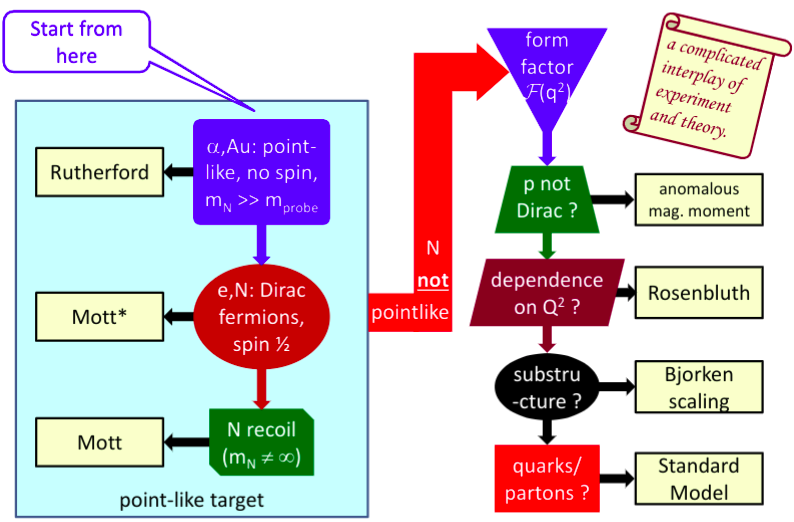
\includegraphics[width=0.7\textwidth]{immagini/fig_treasure_map_scattering}
    \caption{Mappa del tesoro dello scattering.}
    %\label{}
\end{figure}
\subsection{Modello a gas di Fermi}
\begin{itemize}
    \item I nuclei sono stati legati di protoni e neutroni. Il gas di Fermi è un semplice modello.
    \item I protoni e i neutroni sono identici a meno della carica: sono delle sfere con una certa massa; sono fermioni; sono legati all'interno del nucleo, altrimenti sono liberi di muoversi. 
    \item Non consideriamo interazione elettromagnetica, solo nucleare dunque $N=Z=\frac A2$ ed impulso ed energia di Fermi sono uguali per protoni e neutroni (in approssimazione migliore sono differenti gli impulsi). 
    \item Per il principio di indeterminazione ogni $p$ ed $n$ occupano un volume $V=(2\pi\hbar)3$ nello spazio delle fasi.
    \item Dunque abbiamo una buca ben definita identica per protoni e neutroni, e viene rispettata la statistica di Fermi dunque due $p/n$ per livello di energia (con spin opposto).
    \item Da queste approssimazioni possiamo fare dei calcoli semplici:
    \begin{gather*}
    n_n^\uparrow=n_n^\downarrow=n_p^\uparrow=n_p^\downarrow=\frac N2=\frac Z2=\frac A4=\\
    =\frac{[V\_{space}V\_{imp}]\_{TOT}}{[V\_{space}V\_{imp}]\_{ciascuna particella}}=\frac{\frac43\pi r_0^3A\times\frac43\pi p_F^3}{(2\pi\hbar)^3}=\frac{2Ar_0^3p_F^3}{9\pi^2\hbar^3}\implies\\
    \implies N=Z=\frac A2=\frac{4Ar_0^3p_F^3}{9\pi^2\hbar^3}\implies p_F=\frac\hbar{r_0}\sqrt[3]{\frac{9\pi}8}\underset{r_0\approx1.2\,\text{fm}}{\implies}
    \begin{cases}
    p_F\approx250\,\MeV\\
    E_F^{\text{kin}}=\frac{p_F^2}{2m}\approx33\,\MeV
    \end{cases}
    \end{gather*}
    dove il valore di $r_0$ viene da fit del fattore di forma (vedi dopo) e per $E^{\text{kin}}_F$ si è considerata approssimazione non relativistica. 
    \item In conclusione: $V\_{space}\approx\frac43\pi r_0^3A\implies r\_{nucl}\propto A^{1/3}$, impulso ed energia di Fermi non dipendono da $A$ e ad un largo $p_F$ corrisponde bassa energia cinetica ed infine quando $p/n$ sono colpiti da una sonda ($e^\pm/\nu$), se l'energia della sonda è superiore a 30 MeV, si ignora il moto di Fermi.  
\end{itemize}
\subsection{Scattering di Rutherford}
\begin{itemize}
    \item L'esperimento fu eseguito a Manchester nel 1908-1913. Consiste in particelle $\alpha$ contro un bersaglio di oro $Au$.
    \item Propose un modello diverso da quello di J.J. Thompson.
    \item Fu il primo esperimento di scattering di particelle, infatti è la nascita della fisica nucleare.
    \item Dunque si mandarono queste particelle $\alpha$ su un foglio di oro con energia cinetica di qualche MeV. Qualche volta l'angolo di scattering era maggiore di 90$^\circ$ che nella pratica è un evento molto raro ma impossibile se la materia fosse effettivamente omogenea come nel modello di Thompson. L'unica possibile spiegazione è che la materia in realtà è concentrata in piccoli corpi pesanti, i nuclei. Dunque la materia è essenzialmente vuota.
    \item Come modelliamo lo scattering? Rutherford provo con una diffusione a due corpi. Chiaramente solo contributo elettrostatico non relativostico e senza meccanica quantistica. Fu un successo.
    \item Un punto chiave è che il nucleo è abbastanza piccolo da essere visto puntiforme (e con tutta la sua carica) dalla particella $\alpha$ (teorema di Gauss, primo capitolo).
    \item Tuttavia la materia è neutra, ma il fatto è che gli elettroni sono molto leggeri e non possono fermare o deflettere le particelle $\alpha$ perché $m_\alpha\approx8000m_e$.
\end{itemize}
    \subsubsection{Calcolo della sezione d'urto}
    \begin{figure}[H]
        \centering
        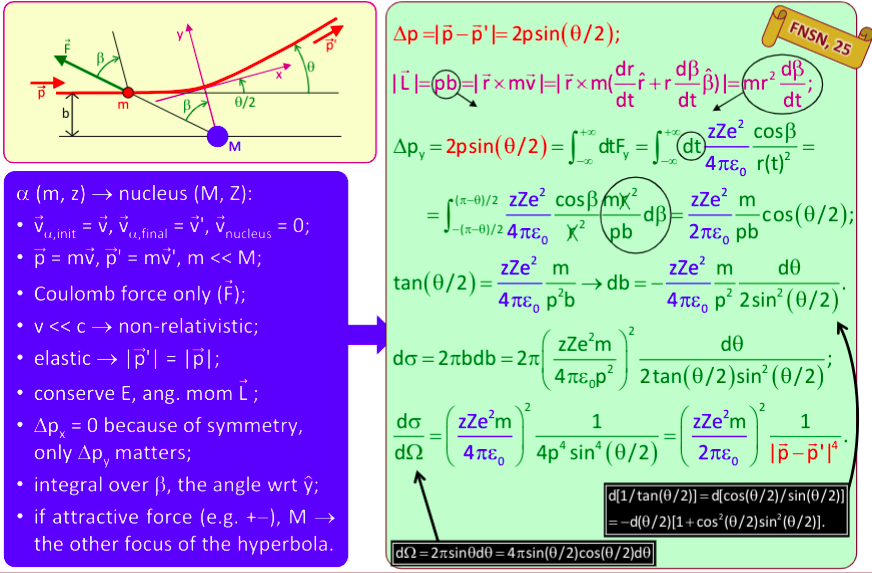
\includegraphics[width=\textwidth]{immagini/fig_rutherford_math.png}
        \caption{$\beta$ è l'angolo tra la particella e l'asse di simmetria (che passa per il punto di minimo approccio).}
        %\label{}
    \end{figure}
    \begin{itemize}
    \item Se la forza è attrattiva la sezione d'urto è uguale perché cambia solo
        \begin{equation*}
    \va F\to -\va F\implies\vartheta\to-\vartheta
    \end{equation*}
    \item Adesso troviamo espressione esplicita per la $r\_{min}$. Cominciamo una particella con $b=0\implies \vartheta=\pi$. Avremo $d_0=r\_{min}(b=0)$ dato da
    \begin{equation*}
    \frac12mv^2=\frac{zZe^2}{4\pi\varepsilon_0d_0}\implies d_0=\frac{zZe^2}{2\pi\varepsilon_0mv^2}\implies \tan\qty(\frac\vartheta2)=\frac{d_0}{2b}
    \end{equation*}
    Per trovare $d$ ($b\neq0$) usiamo conservazione di $\va L$ ed $E$ (dove $v_0$ è la velocità in $d$)
    \begin{equation*}
        \begin{cases}
        mbv=mdv_0\to \frac{v_0}v=\frac bd\\
        \frac12mv^2=\frac12mv_0^2+\frac{zZe^2}{4\pi\varepsilon_0d}=\frac12mv_0^2+\frac12mv^2\frac{d_0}d
        \end{cases}\implies\qty(\frac bd)^2=\qty(\frac{v_0}v)^2=1-\frac{d_0}d\implies 
    \end{equation*}
    \begin{equation*}
        \implies d^2-dd_0-b^2=0\implies d=\dots=\frac{d_0}2\qty(1+\frac1{\sin(\frac\vartheta2)})\implies \dv{\sigma}{\Omega}= \frac{d_0^2}{16\sin^4\qty(\frac\vartheta2)}\overset{\vartheta\to0}{\longrightarrow}\frac{d_0^4}{\vartheta^4}
    \end{equation*}
    \begin{figure}[H]
        \centering
        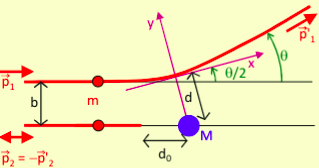
\includegraphics[width=0.6\textwidth]{immagini/fig_ruth_b_nullo.png}
        %\caption{}
        %\label{}
    \end{figure}
    \item Questi calcoli non sono difficili da fare matematicamente, la vera difficoltà è affermare se la materia è omogenea o granulare e vuota.
    \item A grandi $b$ corrispondono piccoli $\vartheta$ a cui corrisponde una divergenza della sezione d'urto, poi comunque non diverge perché c'è un limite dato dalla presenza di altri nuclei di oro. 
    \item Nel 1909 trovarono eventi di backscattering che misero in crisi il modello di Thomson. Era comunque inconsistente perché elettroni che accelerano emettono radiazione elettromagnetica e dovrebbero collassare nel nucleo. Dopo la nascita della MQ comunque la sezione d'urto rimase la stessa\footnote{la prof dice "per caso", Greco dice perché la $\alpha$ ha spin nullo}.
\end{itemize}
\subsubsection{Raggio nucleare}    
Quanto è grande il nucleo? Se la particella $\alpha$ ha una traiettoria esterna, essa non può sondare la sua \textit{ipotetica} struttura interna. Rutherford arrivò a $r\approx10^{-14}$ m. Per andare oltre servono sonde con $E\_{kin}\approx30$ MeV.
\begin{itemize}
    \item $b$ ed $r\_{min}$ non possono essere misurati direttamente per ciascun evento, ma la legge puntiforme di Rutherford (rpl) lega $b\leftrightarrow\vartheta$ infatti a piccoli parametri d'urto corrispondono grandi angoli.
    \item Il teorema di Gauss predice una deviazione da rpl quando l'energia cinetica delle $\alpha$ è grande. Avendo un $r\_{min}<R\_N$ si avrà schermaggio dunque degli angoli $\vartheta$ più piccoli.
    \item nel 1961 fecero una misura di scattering $\alpha$ contro piombo mettendosi a $\vartheta=60^\circ$ ed osservarono una deviazione da rpl per energie superiori a 25 MeV (dunque nucleo non è puntiforme).
    \item Ad angoli grandi, se il bersaglio è puntiforme la sezione d'urto è grande, se invece è esteso la sezione d'urto è minore. Non è proprio chiaro scritto così ma è legato ai precedenti punti. 
\end{itemize}
\subsection{Cinematica}
Come già detto la nostra sonda è una particella elementare e il nostro bersaglio è in generale un complesso sistema adronico. Nello stato finale si avrà la sonda invariata mentre il nucleo in generale cambia:
\begin{enumerate}
    \item Scattering elastico: il nucleo rimane nello stato fondamentale.
    \item Eccitazione: il nucleo nello stato finale si trova in uno stato eccitato.
    \item Nuovo sistema adronico, con $n$ particelle.
\end{enumerate}
L'idea è capire/studiare la struttura degli adroni osservando lo scattering.
\subsubsection{Scattering elastico}
\begin{itemize}
    \item Consideriamo $e^-N\to e^-N$, con nucleo inizialmente a riposo. Allora avremo che l'energia finale dell'elettrone è (da consevazione di quadrimpulso)
    \begin{equation*}
        E'=\frac E{1+\frac EM\qty(1-\cos\vartheta)}=\frac E{1+\frac{2E}{M}\sin^2\frac\vartheta2}\approx \abs{\va p'}
    \end{equation*}
    \begin{figure}[H]
        \centering
        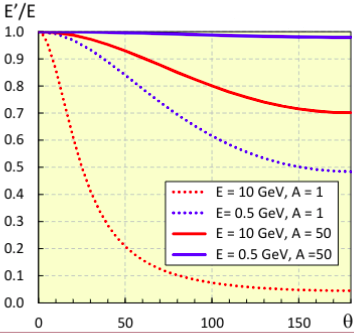
\includegraphics[width=0.6\textwidth]{immagini/fig_frac_energy_scatt.png}
        \caption{Grafico della frazione di energia portata via dall'elettrone. Quando l'energia iniziale è alta e il nucleo è piccolo (A=1) viene trasferita molta energia al nucleo a grandi angoli. Se $\frac EM$ è piccolo, allora $E'\approx E\implies p\_H\approx0$ cioè non rincula ed è indipendente da $\vartheta$.}
        %\label{}
    \end{figure}
    \item Dunque nota l'energia iniziale e fissata la massa $M$ del nucleo, lo stato finale è definito da \textit{una variabile indipendente} $E'$ o $\vartheta$.
    \item Per il calcolo esplicito bisogna considerare la conservazione del quadrimpulso prima e dopo lo scattering, e poi fare il quadrato e sottrarre le due equazioni isolando l'energia del nucleo post-scattering (una per conservazione di energia e l'altra per l'impulso).
    \item Consideriamo l'impulso trasferito $\va q = \va p - \va p'$. Se $E/M$ è piccolo, allora $p'=p\implies \abs{\va q}=2\abs{\va p}\sin\frac\vartheta2$. 
    \item C'è anche la controparte relativistica, ossia il quadrivettore $q=(E-E',\va p-\va p')$. 
    \begin{equation*}
    -q^2=-(2m_e^2-2EE'+2\abs{\va p}\abs{\va p'}\cos\vartheta)\approx4EE'\sin^2\frac\vartheta2=Q^2>0
    \end{equation*}
    Possiamo ricavare una relazione per $Q^2$ nel seguente modo:
    \begin{equation*}
        E'=\frac{EM}{M+2E\sin^2\frac\vartheta2}=\frac{EM}{M+\frac{Q^2}{2E'}}=\frac{2EE'M}{2E'M+Q^2}\implies 2EM=E'M+Q^2\implies
    \end{equation*}
    \begin{equation*}
        \implies Q^2=2M(E-E')\qquad E'=E-\frac{Q^2}{2M}
    \end{equation*}
    \item Vediamo i casi cinematici limite:
    \begin{enumerate}
        \item $\vartheta=0$: $E'=E$, $Q^2=0$.
        \item $\vartheta=\pi$: $E-E'=E\frac{M+2E}{M+2E}-\frac{EM}{M+2E}=\frac{2E^2}{M+2E}$, quindi se $E\ll M$ allora $E-E'\approx E\implies E'\approx0$ 
    \end{enumerate}
    \begin{figure}[H]
        \centering
        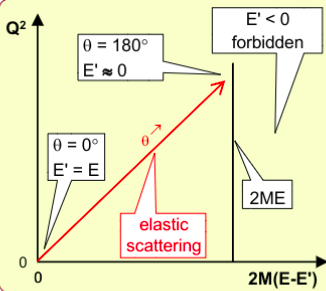
\includegraphics[width=0.6\textwidth]{immagini/fig_q_2_elastic.png}
        \caption{Grafico di $Q^2$ in funzione di $2M(E-E')$: solo un segmento è permesso.}
        %\label{}
    \end{figure}
\end{itemize}
\subsubsection{Perché usare $\abs{\va q}$ o $Q^2$?}
La variabile $\va q$ (o $Q^2$ in regime relativistico) è molto importante
\begin{itemize}
    \item È legata alla lunghezza d'onda di De Broglie della sonda $\slashed\lambda=\frac\hbar{\abs{\va q}}$. Rappresenta la scala dello scattering, ossia strutture più piccole di $\slashed\lambda\sim\frac1{\abs{\va q}}$ non possono essere viste dalla sonda.
    \item Questo viene dal principio di indeterminazione $\Delta p\Delta x\geq \frac\hbar2$.
    \item A grandi $\abs{\va q}$ corrispondono grandi energie, ma l'opposto in generale non è vero: esistono processi ad alta energia e grandi distanze.
    \item La ricerca di scale inferiori porta inevitabilmente a maggiori $Q^2$ e dunque a grandi energie (soldi e risorse). 
\end{itemize}
\subsubsection{Scattering inelastico}
Consideriamo il caso $lN\to l'H$. Sia $p$ il quadrimpulso dell'elettrone, $P$ il quadrimpulso del nucleo, $p'$ il quadrimpulso dell'elettrone dopo lo scattering e $p_H$ il quadrimpulso del nucleo dopo lo scattering. Definiamo/riscriviamo delle variabili Lorentz-invarianti:
\begin{itemize}
    \item $\nu=q\frac PM=E-E'$ è l'energia persa dall'elettrone.
    \item $Q^2=-q^2=2(EE'-pp'\cos\vartheta)-2m^2\approx4EE'\sin^2(\frac\vartheta2)$ 
    \item $x=\frac{Q^2}{2M\nu}$ è la "x di Bjorken" e corrisponde alla frazione di quadrimpulso dell'adrone portata dal partone interagente.
    \item $y=\frac{q\vdot P}{p\vdot P}=\frac\nu E$ è la frazione di energia persa dal leptone nel riferimento del bersaglio.
    \item $W^2=(p\_H)^2=(p+q)^2=M^2-Q^2+2M\nu$ è il quadrato della massa del sistema adronico finale. Se $W=M$ allora si ha scattering elastico.
    \item $s=(q+P)^2=(p'+p\_H)^2\approx M(M+2E)$ è il quadrato dell'energia nel centro di massa.
\end{itemize}
\begin{figure}[H]
    \centering
    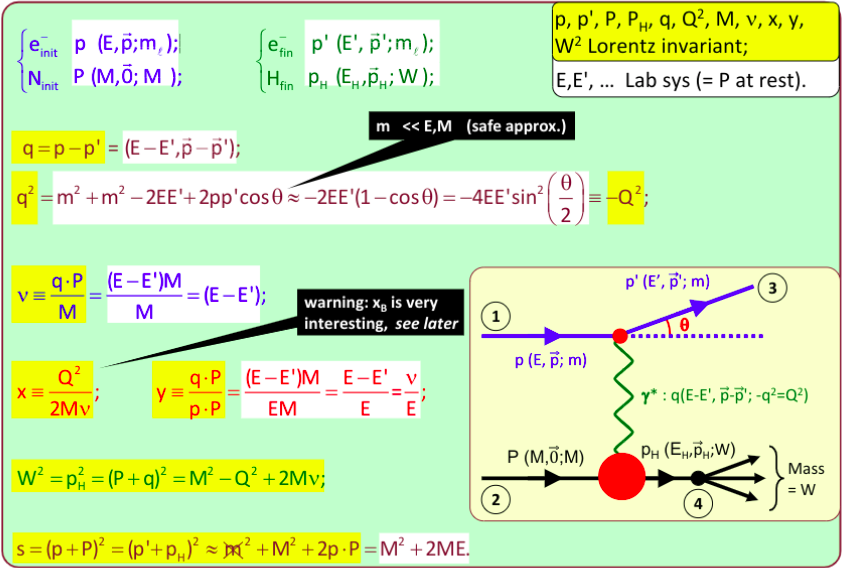
\includegraphics[width=\textwidth]{immagini/fig_conti_kinem.png}
    %\caption{}
    %\label{}
\end{figure}
\begin{itemize}
    \item Nel caso elastico $eN\to eN$, $\nu$ e $Q^2$ NON sono indipendenti:
    \begin{equation*}
    W^2=M^2=(P+q)^2=M^2-Q^2+2M\nu\implies Q^2=2M\nu\implies\frac{Q^2}{2M\nu}=x=1
    \end{equation*}
    \item Dunque ovviamente nel caso elastico c'è solo una variabile indipendente ($E'$ o $\vartheta$), mentre nel caso inelastico ce ne sono due:
    \begin{equation*}
        Q^2=M^2+2M\nu-W^2=2M\nu-(W^2-M^2)\leq2M\nu\implies x\leq1
    \end{equation*}
    se $W$ non è fissato, $Q^2$ e $\nu$ sono indipendenti.
    \item Si scelgono per convenienza le due variabili indipendenti da analizzare, e.g. $(E',\vartheta)$, $(Q^2,\nu)$, $(x,y)$.
\end{itemize}
\subsubsection{Deep inelastic scattering (DIS)}
Torniamo al piano $Q^2,\nu$.
\begin{itemize}
    \item Entrambi sono Lorentz-invarianti.
    \item $Q^2=4EE'\sin^2\frac\vartheta2\geq0$ dunque stiamo nel primo quadrante.
    \item $\nu=E-E'\implies0\leq\nu\leq E$ dunque solo una banda è permessa.
    \item $x=\frac{Q^2}{2M\nu}\leq1\implies 0\leq x\leq1$ dunque solo il "triangolo basso" è permesso.
    \item $y=\frac\nu E\implies0\leq y\leq1$.
    \item $W^2=M^2-Q^2+2M\nu$ la bisettrice $x=1$ definisce lo scattering elastico dove $W=M$. Lungo la bisettrice solo $\vartheta$ varia: $\vartheta=0\implies Q^2=\nu=0$.
    \item Il luogo dei punti $W'^2=$cost sono linee parallele alla bisettrice, alcune di loro definiscono gli stati eccitati.
    \item A distanze maggiori dalla bisettrice abbiamo DIS e potenzialmente nuova fisica.
    \begin{figure}[H]
        \centering
        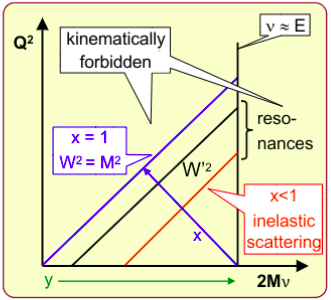
\includegraphics[width=0.6\textwidth]{immagini/fig_dis.png}
        %\caption{}
        %\label{}
    \end{figure}
\end{itemize}
\subsubsection{Riassunto cinematica}
\begin{figure}[H]
    \centering
    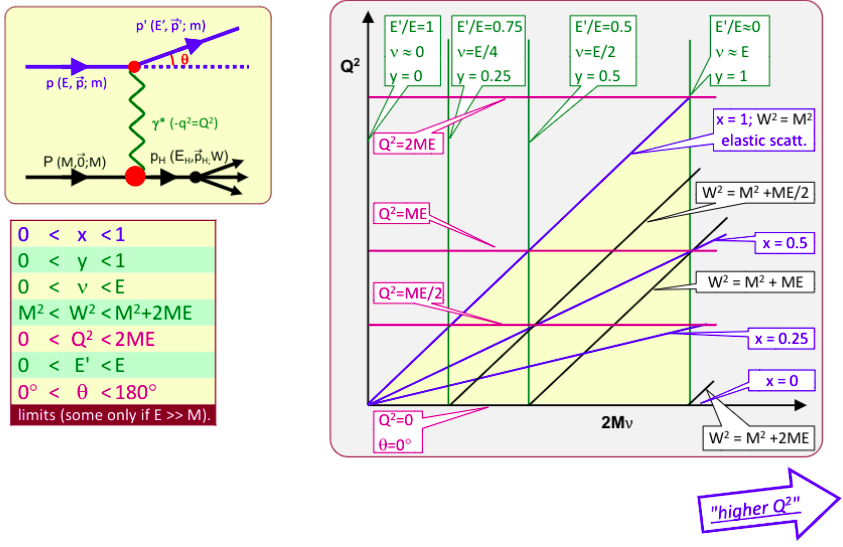
\includegraphics[width=\textwidth]{immagini/fig_kin_summary_hadron.png}
    %\caption{}
    %\label{}
\end{figure}
\subsection{Scattering elastico elettrone-adrone: Rutherford + MQ}
Negli anni 20 entrò in gioco la meccanica quantistica. 
\begin{itemize}
    \item La formula di Rutherford funziona anche in questo caso, considerando il caso non relativistico e la approssimazione di Born.
    \item Il potenziale è comunque coloumbiano.
    \item Gli stati iniziali e finali delle particelle sono onde piane.
    \item Trascuriamo il rinculo.
    \item Il potenziale all'infinito non contribuisce a causa degli altri nuclei.
    \item Vediamo il calcolo:
    \begin{gather*}
        V(r)=-\frac{zZ\alpha}r;\;\va q=\Delta p=\va p-\va p';\;q=\abs{\va q}=2p\sin\frac\vartheta2\\
        \psi_i=\frac1\Phi e^{i\va p\vdot \va r};\;\psi_f=\frac1\Phi e^{i\va p'\vdot \va r};\; \dv{n}{E'}=\frac{4\pi p'^2\Phi}{(2\pi)^3v'}\\
        M\_{fi}=\braket{\psi_f}{V}{\psi_i}=\frac1\Phi\int e^{-i\va p'\vdot\va r}V(r)e^{i\va p\vdot\va r}\dd^3r=\\
        =-\frac1\Phi\iiint \frac{zZ\alpha}re^{i\va q\vdot\va r}r^2\dd r\dd\Omega=-\frac{4\pi}\Phi\frac{zZ\alpha}{q^2}\\
        \implies \dv{\sigma}{\Omega}=\frac1{4\pi}\qty[2\pi\abs{M\_{fi}}^2\dv{n}{E'}\frac\Phi{v'}]\underset{\begin{subarray}{c}
            v'\to c=1\\
            p'=E'
         \end{subarray}}{\longrightarrow}\frac12\abs{\frac{4\pi}\Phi\frac{zZ\alpha}{q^2}}^2\frac{\Phi E'^2}{2\pi^2}\Phi=\frac{4z^2Z^2\alpha^2E'^2}{q^4}
    \end{gather*}
    stesso risultato!
    \item Tuttavia lo scattering $\alpha-$Nucleo ha luogo due particelle non elementari, dunque sostituiamo $\alpha$ con elettrone. 
    \item La dinamica dello scattering $eN$ può essere descritta dalla formula di Rutherford con un aggiustamento dovuto a Mott\footnote{L'asterisco indica che stiamo approssimando trascurando il rinculo del nucleo.}:
    \begin{equation*}
    \dv{\sigma}{\Omega}\_{Mott*}=\dv{\sigma}{\Omega}\_{Ruth}\times\qty(1-\beta^2\sin^2\frac\vartheta2)\underset{\beta=\frac{\abs {\va p}}{E}\to1}{\longrightarrow}\dv{\sigma}{\Omega}\_{Ruth}\cos^2\frac\vartheta2=\frac{4Z^2\alpha^2E'^2}{q^4}\cos^2\frac\vartheta2
    \end{equation*}
    \item Come la formula di Rutherford, la sezione d'urto di Mott trascura le dimensioni del nucleo, se ci sono (e anche il rinculo quando mettiamo *).
    \item Al contrario della formula di Rutherford, qui si tiene conto dello spin ($\frac12$) degli elettroni.
\end{itemize}
\subsubsection{Elicità}
\begin{itemize}
    \item Il fattore $\cos^2\frac\vartheta2$ nella sezione d'urto di Mott viene dalla equazione di Dirac. Lo si capisce considerando il caso estremo $\vartheta\sim\pi$.
    \item Per particelle relativistiche ($\beta\to1$) l'elicità $h$ (proiezione di spin su impulso) è conservata:
    \begin{equation*}
    h=\frac{\va s\vdot \va p}{\abs{\va s}\abs{\va p}}
    \end{equation*}
    \item La conservazione richiede uno spin flip dell'elettrone tra stato iniziale e finale, perché anche l'impulso flippa a 180$^\circ$.
    \item Però in questa condizione, il momento angolare NON si conserva se il nucleo non assorbe la variazione di spin (e.g. perché è a spin nullo). Dunque lo scattering a $\vartheta\approx\pi$ è proibito.
    \item Il fattore $\cos^2\frac\vartheta2$ nella formula di Mott è connesso allo spin e descrive la parte magnetica della interazione. Quindi questo termine serve ad annullare la sezione d'urto altrimenti non si conserverebbe il momento angolare.
    \item Se invece il target ha spin, la proiezione dello spin dell'elettrone può cambiare perché la conservazione del momento angolare può essere compensata dal cambio nella direzione dello spin del bersaglio. In questo caso lo scattering a 180$^\circ$ è possibile.
    \begin{figure}[H]
        \centering
        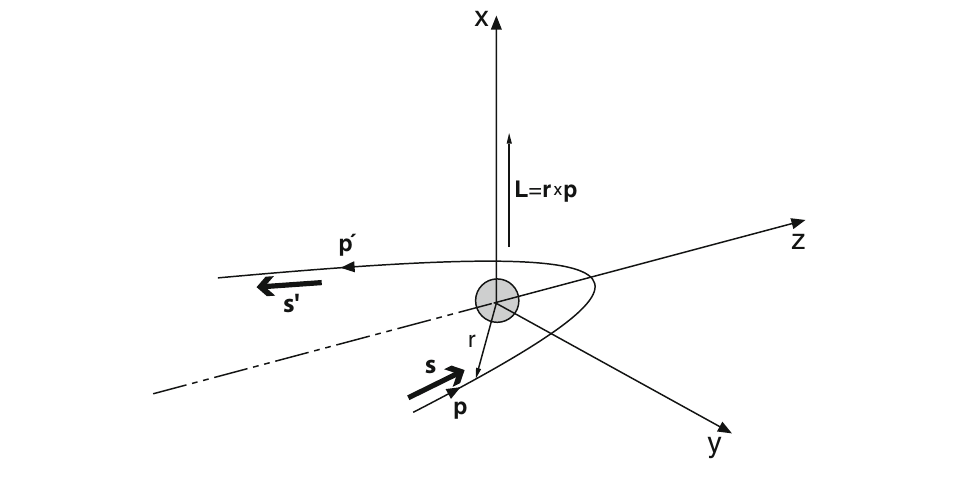
\includegraphics[width=0.8\textwidth]{immagini/fig_elic_mott.png}
        \caption{L'elicità si conserva nel limite $\beta\to1$. Questo significa che la proiezione dello spin lungo $z$ deve cambiare di segno nello scattering a 180$^\circ$. Questo è impossibile se il bersaglio è a spin nullo per conservazione del momento angolare.}
        %\label{}
    \end{figure}
\end{itemize}
\subsubsection{L'esperimento}
L'esperimento è consistente con la cinematica dello scattering elastico? Abbiamo i dati $e+\,^{12}C$.
\begin{figure}[H]
    \centering
    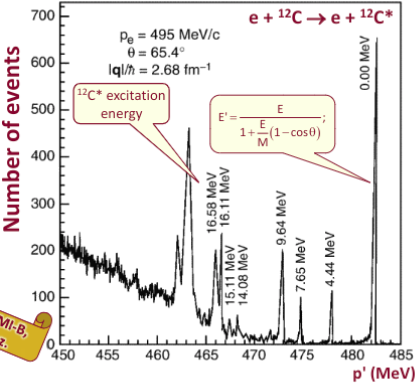
\includegraphics[width=0.6\textwidth]{immagini/fig_plot_eN_scatt.png}
    %\caption{}
    %\label{}
\end{figure}
Il plot dei numeri di eventi con $E\_{in}$ e $\vartheta$ fissato, mostra vari picchi:
\begin{enumerate}
    \item Il più grande è il picco elastico come ci aspettiamo ($E'\approx p'=482$ MeV)
    \item Si ha una struttura "ricca" a causa dello scattering anelastico in cui si porta il carbonio a stati eccitati.
    \item Quindi ok la cinematica, tutto torna ed è spiegabile. Ma la dinamica? Dobbiamo misurare $\dv{\sigma}{\Omega}$ in funzione di $\vartheta$.
\end{enumerate}
\subsection{Fattore di forma}
\begin{itemize}
    \item La sezione d'urto sperimentale è in accordo con quella di Mott solo per bassi angoli, cioè per bassi $\abs{\va q}$. 
    \item Ad un certo punto l'andamento devia da $\vartheta^{-4}$, probabilmente la ragione è la struttura del nucleo, che risulta in una carica effettiva minore vista dal proiettile (teorema di Gauss).
    \item Consideriamo la densità di carica:
    \begin{equation*}
    \rho(\va x)=Zef(\va x),\quad \int f(\va x)\dd^3x=1
    \end{equation*}
    allora definiamo \textit{fattore di forma} $F(\va q)$ la trasformata di Fourier della distribuzione di carica:
    \begin{equation*}
        F(\va q)=\int e^{i\frac{\va q\vdot\va x}\hbar}f(\va x)\dd^3{x};\quad \va q=\va p-\va p'
    \end{equation*}
    se è puntuale allora $f(\va x)=\delta(\va x)\implies F(\va q)=1$.
    \item Se $\rho(\va x)$ dipende solo dal modulo $\abs{vec x}$ allora
    \begin{equation*}
        \dv{\sigma}{\Omega}\_{sperimentale}=\dv{\sigma}{\Omega}\_{Mott}\times\abs{F(q^2)}^2
    \end{equation*}
    e i fattori di forma sono misurabili, almeno in principio.
    \begin{figure}[H]
        \centering
        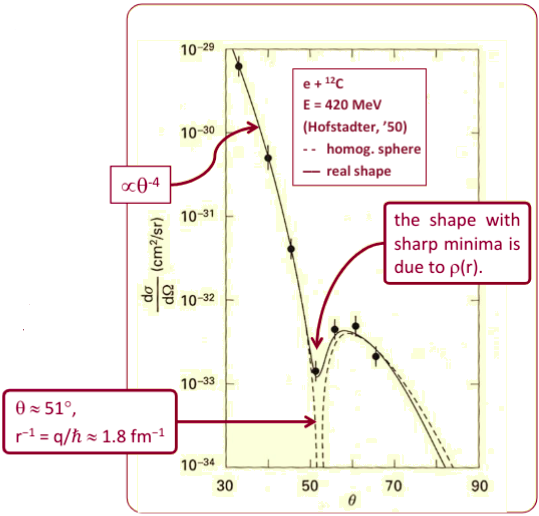
\includegraphics[width=0.6\textwidth]{immagini/fig_sigma_theta_en.png}
        %\caption{}
        %\label{}
    \end{figure}
    \item Vediamo il calcolo quantistico ($\va{R} = \va{r} - \va{r}'$):
    \[
    V(\va{r}) = -\int d^3r' \frac{Z \alpha f(\va{r}')}{4 \pi |\va{r} - \va{r}'|}
    \]

    \[
    \psi_i = \frac{e^{i \va{p} \vdot \va{x} - E t}}{\sqrt{\Phi}}; \quad \psi_f = \frac{e^{i \va{p}' \vdot \va{x} - E t}}{\sqrt{\Phi}}
    \]

    \[
    M_{fi} = \langle \psi_f | V(\va{r}) | \psi_i \rangle = \frac{1}{\Phi} \int e^{-i \va{p}' \vdot \va{r}} V(\va{r}) e^{i \va{p} \vdot \va{r}} d^3r =
    \]

    \[
    = -\frac{1}{\Phi} \int \int e^{i \va{q} \vdot \va{r}} \frac{Z \alpha f(\va{r}')}{4 \pi |\va{r} - \va{r}'|} d^3r' d^3r =
    \]

    \[
    = -\frac{1}{\Phi} \int \int e^{i \va{q} \vdot (\va{r}-\va r')}e^{i\va q\vdot \va r'} \frac{Z \alpha f(\va{r}')}{4 \pi |\va{r} -\va r'|} \dd^3r' \dd^3r =
    \]

    \[
    = \left[-\frac{1}{\Phi} \int e^{i \va{q} \vdot \va{R}} \frac{Z \alpha}{4 \pi |\va{R}|} d^3R \right] \times \left[ \int f(\va{r}') e^{i \va{q} \vdot \va{r}'} d^3r' \right]
    \]

    \[
    = M_{fi}^{\text{point}} \times F(q^2)
    \]

    \[
    \left(\frac{d\sigma}{d\Omega}\right)_{\text{non-point}} = \left(\frac{d\sigma}{d\Omega}\right)_{\text{point}} \times |F(q^2)|^2
    \]
\end{itemize}
\subsubsection{Simmetria radiale}
\begin{itemize}
    \item La funzione $\rho(r)$ potrebbe essere calcolata misurando $F(q^2)$ e poi numericamente faccio integrale
    \begin{equation*}
    \rho(r)=\frac{Ze}{\qty(2\pi)^3}\int F(q^2)e^{-i\va q\vdot\va r}\dd^3q
    \end{equation*}
    \item Tuttavia, il range di valori di $q$ accessibili dagli esperimenti è limitato. Dunque il comportamento di $F(q^2)$ per grandi $q^2$ (i.e. piccole distanze, la regione di interesse) deve essere estrapolata sotto ragionevoli assunzioni. 
    \item Si può calcolare per il caso simmetrico trascurando il rinculo nucleare.
    \begin{equation*}
    F(q^2)=\int e^{i\va q\vdot\va r}f(r)\dd^3r=2\pi\int_0^\infty r^2f(r)\dd r\int_{-1}^1e^{iqr\cos\theta}\dd(\cos\theta)=\dots=4\pi\int_0^\infty r^2f(r)\frac{\sin(qr)}{qr}\dd r
    \end{equation*} 
\end{itemize}
\subsubsection{Esempi di fattori di forma}
Avendo
\begin{equation*}
f(r)=\frac1{(2\pi)^3}\int F(q^2)e^{-iqr}\dd^3q\qquad F(q^2)=4\pi\int_0^\infty r^2f(r)\frac{\sin(qr)}{qr}\dd r
\end{equation*}
\begin{figure}[H]
    \centering
    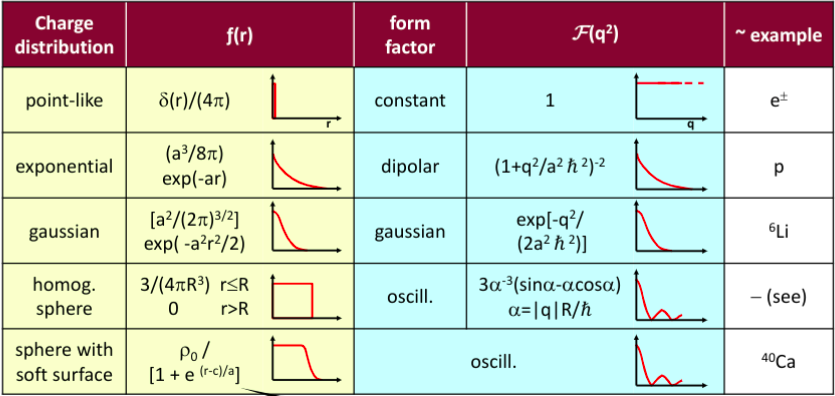
\includegraphics[width=0.6\textwidth]{immagini/fig_factor_form_example.png}
    %\caption{}
    %\label{}
\end{figure}
\subsubsection{Sfera omogenea}
\begin{itemize}
    \item Consideriamo una densità
    \begin{equation*}
        \rho(r)=f(r)=
        \begin{cases}
            \rho_0=\frac3{4\pi R^3} & r\leq R\\
            0 & r>R
        \end{cases}
    \end{equation*}
    Avremo
    \begin{equation*}
    F(q^2)=4\pi\int_0^\infty f(r)r^2\frac{\sin(qr)}{qr}\dd r=\dots=\frac 3{q^3R^3}\qty(\sin(qR)-qR\cos(qR))
    \end{equation*}
    \item Il primo minimo si ha per $qR=\tan(qR)\implies qR\approx4.5$ e confrontandolo con l'esperimento di $^{12}$C con $q\approx1.8\,$ fm$^{-1}$ otteniamo:
    \[ 
    R\approx4.5\, \text{r}\_{min}=\frac{4.5}{1.8}\approx2.5\, \text{fm}
    \] 
    cioè $^{12}$C è approssimativamente una sfera di raggio 2.5 fm.
    \begin{figure}[H]
        \centering
        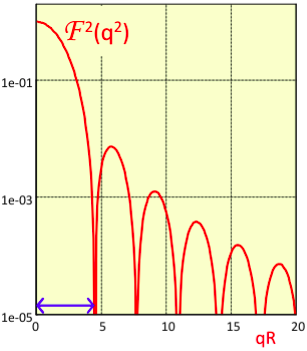
\includegraphics[width=0.4\textwidth]{immagini/fig_min_F_q.png}
        %\caption{}
        %\label{}
    \end{figure}
    \item Si può studiare il comportamento per $q\to0$ sviluppando in serie il termine $e^{iqr\cos\vartheta}$ dentro l'integrale ottenendo
    \begin{equation*}
    F(q^2)=\iiint e^{iqr\cos\vartheta}f(r)r^2\dd r\dd{\cos\vartheta}\dd\phi =\dots=1-\frac16q^2\expval{r^2}+\dots\implies r\_{RMS}=\sqrt{\expval{r^2}}=\sqrt{-6\dv{F(q^2)}{q^2}\Big|_{q^2=0}}
    \end{equation*}
    il parametro $\expval{r^2}$ è una misura della dimensione al quadrato della  (carica della) particella. Per una sfera omogenea $\expval{r^2}=\frac35R^2$.
\end{itemize}
\subsubsection{Casi limite $q\to0$ e $q\to\infty$}
\begin{itemize}
    \item $q$ è approssimativamente la variabile coniugata di $b$, il parametro d'impatto. Quindi per $q$ molto bassi ($b$ molto grandi) il bersaglio è come se fosse puntiforme; per $q$ meno bassi ($b$ meno grandi) il bersaglio si comporta come una sfera omogenea; per $q$ molto alti si può sondare il nucleo a piccole distanze.
    \item La "nuova fisica" (cioè nuove nuove sub-strutture) richiede $q$ molto alti, che è possibile solo se il proiettile ha energia molto elevata. 
    \item La storia si ripete più volte, da Rutherford al LHC, ma con $b$ inferiori (i.e. $q$ più alti). Per questo servono acceleratori sempre più potenti.
\end{itemize}
\subsubsection{Riepilogo fattore di forma}
\begin{itemize}
    \item I nuclei pesanti non sono sfere omogenee con bordo netto, ma piuttosto con un bordo leggero. 
    \item La distribuzione di carica è ben riprodotta dalla Wood-Saxon
    \begin{equation*}
    \rho\_{carica}(r)=\frac{\rho_0}{1+e^{\frac{r-c}a}}\qquad c\approx1.07\,\text{ fm}\times A^{\frac13}\text{ (raggio)}\;a\approx0.54\text{ fm (pelle)}
    \end{equation*}
    \item Per i nuclei leggeri l'andamento è più gaussiano.
    \item Tutti i nuclei hanno simmetria sferica, solo i lantanidi (terre rare) sono più ellissoidali.
\end{itemize}
\subsection{Scattering e-N: energie superiori}

\noindent
\begin{minipage}[t]{0.48\textwidth}
    \begin{itemize}
        \item Sondare scale spaziali più piccole richiede energie maggiori, sia nello stato iniziale che finale (gli esperimenti odierni operano alla scala del TeV cioè  
        $\sim10^{-18}$ m = 10$^{-3}$ fm). 
        \item Correzioni di alta energia + meccanica quantistica alla formula di Rutherford consistono in:
        \begin{enumerate}
            \item Considerare lo spin dell'elettrone, perché Rutherford aveva solo bosoni (già discussa)
            \item Includere il rinculo del bersaglio nella sezione d'urto di Mott.
            \item utilizzare i quadrivettori $p$ e $p'$ per descrivere lo scattering, invece dei vettori tradizionali.
            \begin{equation*}
            Q^2=4EE'\sin^2\frac\vartheta2
            \end{equation*}
            \item Per lo scattering $eN$, considerare il momento magnetico dei nucleoni, introducendo il parametro $\tau =\frac{ Q^2}{4M^2}$.
        \end{enumerate}
    \end{itemize}
\end{minipage}
\hfill
\begin{minipage}[t]{0.48\textwidth}
    \begin{figure}[H]
        \centering
        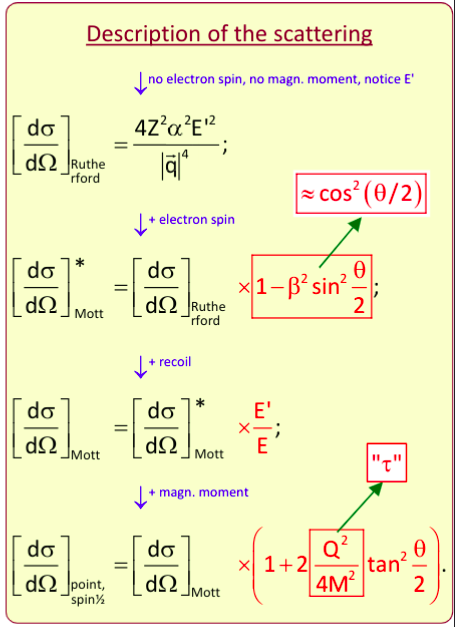
\includegraphics[width=\textwidth]{immagini/fig_sez_urto_varie.png}
        %\caption{}
        %\label{}
    \end{figure}
\end{minipage}
\subsubsection{Momenti magnetici}
\begin{itemize}
    \item Per particelle di massa $m$, carica $e$, puntiformi e $s=\frac12$, l'equazione di Dirac assegna loro un momento di dipolo magnetico
    \begin{gather*}
    \mu_C=\frac{ge\hbar}{4m}\\
    g=\text{ rapporto giromagnetico }=2
    \end{gather*}
    \item Una particella idea di Dirac ha momento di dipolo magnetico pari a 
    \[
    \mu_e=\frac{e\hbar}{2m_e}\approx 5.79\times10^{-5}\frac{eV}T
    \]
    \item La prima misurò confermo questo valore.
    \item Per particelle neutre $\mu_N=0$.
    \item Questo effetto aggiunge alla sezione d'urto un termine, corrispondente alla probabilità di spin flip, proporzionale a: 
    \begin{enumerate}
    \item $\sin^2\frac\vartheta2$
    \item $\frac1{\cos^2\frac\vartheta2}$ per rimuovere la dipendenza da non-flip.
    \item $\mu_N^2\propto\frac1 {M^2}$
    \item $Q^2$ (quadrato de campo magnetico indotto dall'elettrone)
    \end{enumerate}
    \begin{equation*}
        (\dv{\sigma}{\Omega})_{\begin{subarray}{c}
            \text{puntiforme}\\
            \text{spin }\frac12
         \end{subarray}}=(\dv{\sigma}{\Omega})\_{Mott}\times\qty(1+2\frac{Q^2}{4M^2}\tan^2\frac\vartheta2)
    \end{equation*}
    \item Dunque lo spin-flip è particolarmente rilevante a grandi $Q^2$ e grandi $\vartheta$.
\end{itemize}
\subsubsection{Momenti magnetici anomali}
\begin{itemize}
    \item Il magnetismo nucleare è una combinazione dei momenti magnetici intrinseci dei nucleoni e dei loro moti orbitali relativi.
    \item Tutti i nuclei con $Z$ pari e $N$ pari hanno $\mu_{\text{nuclei}} = 0$.
    \item Si definisce per i nucleoni (protone e neutrone) il valore di Dirac:
    \[
    \mu_N = \frac{e\hbar}{4m_N} \approx 3.1525 \times 10^{-14} \, \text{MeV/T}.
    \]
    \item Se $p$ e $n$ fossero particelle di Dirac ideali, avrebbero:
    \[
    \mu_p = 2\mu_N, \quad \mu_n = 0
    \]
    cioè, nella notazione convenzionale:
    \[
    \frac{g_p}{2} = \frac{\mu_p}{\mu_N} = 1, \quad \frac{g_n}{2} = 0
    \]
    \item Tuttavia, gli esperimenti hanno rilevato anomalie:
    \[
    \frac{g_p}{2} = +(2.7928473508 \pm 0.0000000085), \quad 
    \frac{g_n}{2} = -(1.91304273 \pm 0.00000045).
    \]
    \item Pertanto, esistono altri effetti che contribuiscono ai momenti magnetici, ovvero $p$ e $n$ \textbf{non sono} particelle puntiformi ideali di spin $\frac{1}{2}$ di Dirac. 
    \item Forse non sono nemmeno puntiformi.
    \item In tal caso, il loro $g$ è dovuto alla loro struttura interna (potenzialmente complessa), in analogia con il caso nucleare.
\end{itemize}
\subsubsection{Sezione d'urto di Rosenbluth}
\begin{itemize}
    \item Nello scattering $eN$, il contributo principale è dato dallo scambio di un singolo fotone.
    \item Il vertice $ee\gamma^*$ è ben compreso, con tre particelle puntiformi e ben studiate.
    \item Al contrario, il vertice $NN'\gamma^*$ è la parte sconosciuta, a causa della struttura interna del protone.
    \item Strategia:
    \begin{itemize}
        \item assumere un processo più semplice ($N =$ fermione di Dirac),
        \item confrontarlo con gli esperimenti,
        \item quindi modificare la teoria, inserendo parametri che modellano la struttura del nucleone.
    \end{itemize}
    \item Si tiene anche conto dello spin e del momento magnetico, sia dell'elettrone che del nucleone.
    \item Si "generalizza" la sezione d'urto definendo la \textbf{sezione d'urto di Rosenbluth}, funzione di \textbf{due fattori di forma}, entrambi dipendenti da $Q^2$:
    \begin{itemize}
        \item $G_E(Q^2)$ per la parte elettrica (senza flip dello spin);
        \item $G_M(Q^2)$ per la parte magnetica (con flip dello spin).
    \end{itemize}
    [In precedenza: $G_E(Q^2) = F(Q^2)$, nessun $G_M$].
    \item Per un fermione di Dirac carico $f_D$, protone, neutrone:
    \begin{itemize}
        \item $f_D$: $G_E^f(Q^2) = 1$, $G_M^f(Q^2) = 1$;
        \item protone ($p$): $G_E^p(Q^2 = 0) = 1$, $G_M^p(Q^2 = 0) \approx 2.79$;
        \item neutrone ($n$): $G_E^n(Q^2 = 0) = 0$, $G_M^n(Q^2 = 0) \approx -1.91$.
    \end{itemize}
\end{itemize}
\begin{gather*}
    (\dv\sigma\Omega)\_{Rosenbluth}=(\dv\sigma\Omega)\_{Mott}\times\qty(\frac{G_E^2+\tau G_M^2}{1+\tau}+2\tau G_M^2\tan^2\frac\vartheta2)\\
    \tau=\frac{Q^2}{4M^2}\qquad G_E=G_E(Q^2)\qquad G_M=G_M(Q^2)
\end{gather*}
\begin{itemize}
    \item La formula di Rosenbluth è un particolare tipo di relazione matematico-logica:
    \begin{itemize}
        \item È un modello che include alcuni vincoli (ad esempio, la dipendenza da $\vartheta$ non può essere modificata);
        \item Ma è "aperta" (ad esempio, $G_E$ e $G_M$ dipendono dalla sconosciuta struttura del nucleone);
        \item Non contiene in sé un pieno potere predittivo;
        \item Tuttavia è un potente strumento di lavoro per studiare i fenomeni e incorporare nuove conoscenze in una teoria (quasi-)formale.
    \end{itemize}
    \item È un approccio di "frontiera", piuttosto comune nella ricerca moderna, che richiede attenzione da parte di chi lo utilizza (studenti e ricercatori).
\end{itemize}
\subsection{Struttura del protone}
\subsubsection{Apparati sperimentali}
Ero assente (slide senza testo)
\subsubsection{Controlli di qualità}
Nel 1956 lo spettrometro di Hofstadter misurò la collisione elastica $ep\to ep$. Misurò $\vartheta$ nel range $35^\circ-138^\circ$ e dunque $Q^2$ tramite le solite relazioni
\begin{gather*}
    E'=\frac E{1+\frac EM(1-\cos\vartheta)}\\
    Q^2=2EE'(1-\cos\vartheta)
\end{gather*}
I controlli di qualità furono fatti verificando questa relazione. Delle misure di $E'$ con $E$ e $\vartheta$ fissate (vari angoli) erano in accordo con le previsioni. Dunque la cinematica in $ep\to ep$ è sotto controllo e possiamo studiare la dinamica.
\subsubsection{Risultati $\dv\sigma\Omega$}
Studiamo la sezione d'urto nel laboratorio.\newline
% Colonne con minipage
\noindent
\begin{minipage}[t]{0.48\textwidth}
    \begin{itemize}
        \item A piccoli angoli, (cioè piccoli $Q^2$ che vuol dire che $\dv\sigma\Omega$ è indipendente da $G_M$) tutte le formule sono d'accordo, dunque $G_E(Q^2=0)\approx1$
        \item A grandi angoli (grandi $Q^2$, piccole distanze e $\dv\sigma\Omega$ dipende da $G_M$) si ha un disaccordo con ogni predizione teorica. Abbiamo valori sbagliati di $G_E$ e $G_M$?
        \item Il disaccordo con (a) e (b) fu previsto (perché protone $g_p\neq2$)
        \item Il disaccordo con (c) mostra una dipendenza da $Q^2$ che significa che il protone non è puntuale.
        \item Hofstadter misurò raggio medio di protone e $\alpha$.  
    \end{itemize}
\end{minipage}
\hfill
\begin{minipage}[t]{0.48\textwidth}
    \begin{figure}[H]
        \centering
        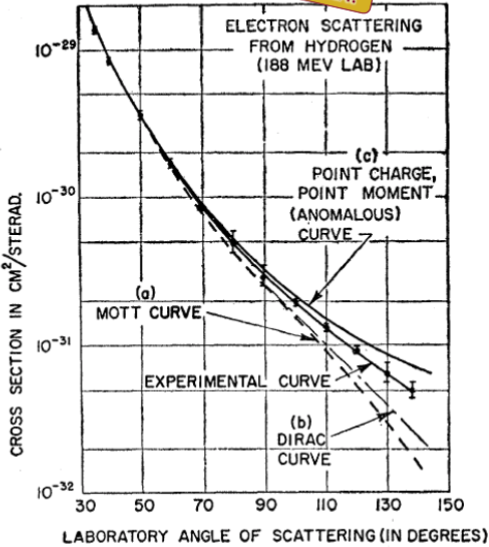
\includegraphics[width=\textwidth]{immagini/fig_proton_structure_result.png}
        \caption{\textit{Rev. Mod Phys., 28, 214.}}
    \end{figure}
\end{minipage}
\begin{center}
    \begin{tabular}{|c|c|c|c|c|}
        \hline
        & \textbf{(a) Mott} & \textbf{(b) Dirac} & \textbf{(c) A-Dirac} & \textbf{(d) Exp.} \\
        \hline
        $G_E$ & 1 & 1 & 1 fix & $G_E(Q^2) \approx 1$ \\
        \hline
        $G_M$ & no & 1 & 2.79 fix & $G_M(Q^2)$? \\
        \hline
        \textbf{point-like p?} & yes & yes & "yes"? & no \\
        \hline
        \textbf{fit low $Q^2$?} & yes & yes & no & def. \\
        \hline
        \textbf{fit high $Q^2$?} & no & no & no & def. \\
        \hline
    \end{tabular}
    \end{center}
\subsubsection{$G_{E,M}^{p,n}$ vs $Q^2$}
Ricordiamo la formula di Rosenbluth, a $Q^2$ fissato:
\begin{equation*}
    \frac {(\dv{\sigma}{\Omega})\_{Rosenbluth}}{(\dv{\sigma}{\Omega})\_{Mott}}=\qty(\frac{G_E^2+\tau G_M^2}{1+\tau}+2\tau G_M^2\tan^2\frac\vartheta2)
\end{equation*}
\begin{itemize}
    \item Rapporto in funzione di $E,\vartheta,Q^2$ fissato è dunque del tipo $A+B\tan^2\frac\vartheta2$.
    \item Misura $A$ e $B$ per diversi $Q^2$ in funzione di $\tan^2\frac\vartheta2$. 
    \item Estraiamo $G_E^p, G_M^p$ e $G_E^n, G_M^n$ per $Q^2$ fissato. 
    \item I fattori di forma elettrici e magnetici tendono a una funzione universale di $Q^2$ con forma dipolare:
    \begin{equation*}
    G_E^p(Q^2)\approx \frac{G_M^p}{2.79}\approx \frac{G_M^n}{-1.91}\approx G(Q^2)=\frac1{(1+\frac{Q^2}{A^2})^2}\qquad A^2\approx0.71\GeV^2
    \end{equation*} 
    \item Dalla curva è possibile derivare la funzione $\rho(r)$ a piccoli $Q^2$. Risulta
    \begin{equation*}
    \rho(r)\approx\rho_0e^{-\alpha r},\quad a\approx4.27\,\text{fm}^{-1}
    \end{equation*}
    \item I nucleoni NON sembrano puntiformi o sfere omegenee, ma un sistema non omogeneo diffuso.
    \item Dai valori per $Q^2=0$ abbiamo
    \begin{equation*}
    \expval{r^2}\_{dipole}=-6\hbar^2\dv{G(q^2)}{q^2}\Big|_{q^2=0}=\frac{12}{a^2}\approx0.66\,\text{fm}^2\implies \sqrt{\expval{r^2}\_{dipole}}\approx0.81\,\text{fm}
    \end{equation*}
    \item Notiamo che 
    \begin{gather*}
        \frac {(\dv{\sigma}{\Omega})\_{Rosenbluth}}{(\dv{\sigma}{\Omega})\_{Mott}}=\qty(\frac{G_E^2+\tau G_M^2}{1+\tau}+2\tau G_M^2\tan^2\frac\vartheta2);\quad \tau=\frac{Q^2}{4M^2}\\
        \text{dunque }\lim_{Q^2\to0} {\qty(\dv{\sigma}{\Omega})\_{Rosenbluth}}= \qty(\dv{\sigma}{\Omega})\_{Mott}
    \end{gather*}
    \item Il fattore di forma dei nucleoni mostrano tre differenti intervalli:
    \begin{itemize}
        \item $Q^2\ll m_p^2$: $\tau$ piccolo, $G_E$ domina la sezione d'urto. In questo range misuriamo il raggio medio della carica elettrica $\expval{r\_E}=0.85\pm0.02$ fm.
        \item $0.02\leq Q^2\leq3$ GeV$^2$: $G_E$ e $G_M$ sono entrambi importanti. 
        \item $Q^2>3$ GeV$^2$: $G_M$ domina la sezione d'urto. 
    \end{itemize}
    \item Notiamo che se il protone fosse puntuale, si avrebbe
    \begin{equation*}
    G_E^p(Q^2)=G_M^p(Q^2)=1, \text{ indipendente da }Q^2
    \end{equation*}
    e non si spiega perché "2.79".
    \begin{figure}[H]
        \centering
        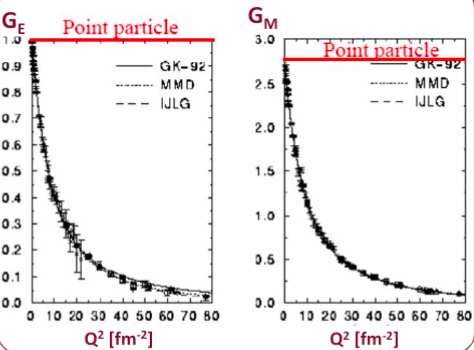
\includegraphics[width=0.6\textwidth]{immagini/fig_G.png}
        %\caption{}
        %\label{}
    \end{figure}
\end{itemize}
Differenze tra nuclei e nucleoni:
\begin{itemize}
    \item I nuclei esibiscono minimi e massimi di diffrazione. Questo fatto corrisponde ad una distribuzione di carica simile alla sfera omogenea con pelle sottile.
    \item I nucleoni hanno fattori di forma diffusi e con distribuzione dipolare: la carica scende esponenzialmente col raggio.
    \item A questo livello, non è chiaro se i nucleoni hanno sottostrutture. Dunque servono esperimenti a piccoli valori di distanza (grandi $Q^2$).
    \item Forse la struttura del nucleone nello scattering elastico, descritta dalla formula di Rosenbluth, è una media con risoluzione insufficiente
    \item A $Q^2$ maggiori ci aspettiamo una varietà di fenomeni:
    \begin{itemize}
        \item Scattering elastico: $ep\to ep$
        \item Eccitazione: $ep\to ep^*$ (e.g. $ep\to e\Delta^+,\,\Delta^+\to p\pi^0$)
        \item Nuovi stati: $ep\to eX^+$ (con $X^+$ sistema di molte particelle)
    \end{itemize}
\end{itemize}
\subsubsection{Maggiore $Q^2$: $H_2=O$}
Si mandano elettroni a 246 MeV contro del vapore acqueo. Lo scattering mostra una distribuzione complessa, con diversi fenomeni nello stesso plot. Ad un certo angolo fissato di elettroni nello stato finale, aumentando $E'$:
\begin{itemize}
    \item $ep\to e\Delta^+$ Eccitazione del protone dell'idrogeno.
    \item $ep/n\to ep/n$ elastico sui nucleoni dell'ossigeno.
    \item $ep\to ep$ elastico sull'idrogeno, con $E'\approx160$ MeV.
    \item $ep\to eX^+$ eccitazioni nucleari.
    \item $e\,^{16}O\to e\,^{16}O$ eccitazioni nucleari o scattering elastico.
\end{itemize}
La distribuzione dipende anche dall'energia dell'elettrone $E$ e dall'angolo dello stato finale $\vartheta$.
\begin{equation*}
    E'=\frac{M^2+2ME-W^2}{2\qty[M+2E\sin^2\frac\vartheta2]}
\end{equation*}
\begin{figure}[H]
    \centering
    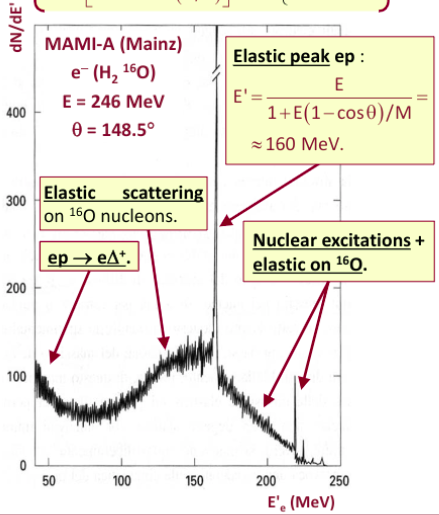
\includegraphics[width=0.6\textwidth]{immagini/fig_higher_q2_water.png}
    %\caption{Distribuzione complessa dello scattering $e$-$H_2O$ a 246 MeV.}
    %\label{}
\end{figure}
\subsubsection{Maggiore $Q^2$: $^4$He, $\vartheta=45^\circ$}
Hofstadter nel 1956 fece un altro di questi esperimenti.
\begin{figure}[H]
    \centering
    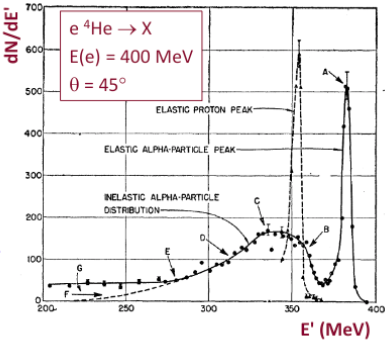
\includegraphics[width=0.6\textwidth]{immagini/fig_higher_q2_helium.png}
    %\caption{Distribuzione complessa dello scattering $e$-$^4$He$ a 246 MeV.}
    %\label{}
\end{figure}
\begin{itemize}
    \item [A.] Il picco elastico $e\,^4$He è ok come previsto. 
    \item [BCDEF.] Lo scattering elastico $ep/en$, con $p/n$ considerati liberi nell'elio (forse inaspettato ma comprensibile); notiamo che la larghezza del picco è dovuta al moto di Fermi dei nucleoni dentro al nucleo. 
    \item [G] La produzione di $\pi^-$ (i.e. di $\Delta$) aumenta la sezione d'urto che altrimenti sarebbe F. Notiamo che minore $E'$, maggiore è il trasferimento di energia.
\end{itemize}
\subsubsection{Maggiore $Q^2$: $^4$He, $\vartheta=60^\circ$}
\begin{figure}[H]
    \centering
    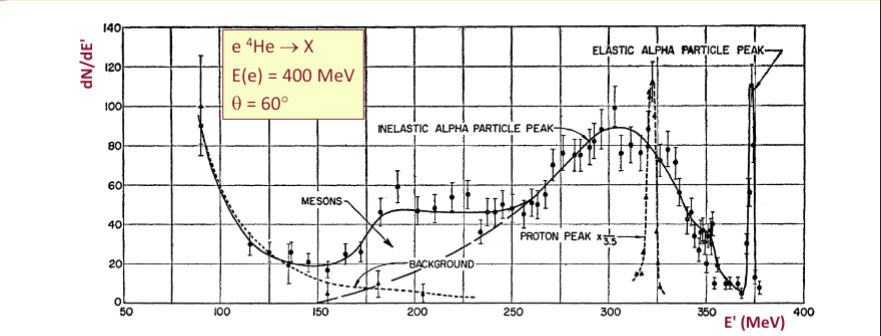
\includegraphics[width=.9\textwidth]{immagini/fig_higher_q2_60.png}
    %\caption{Distribuzione complessa dello scattering $e$-$^4$He$ a 246 MeV con $\vartheta=60^\circ$.}
    %\label{}
\end{figure}
Come prima, ma $\vartheta=60^\circ$, cioè maggiore $Q^2\approx4EE'\sin^2\frac\vartheta2$. Notiamo varie cose\dots
\begin{itemize}
    \item Il picco elastico è minore, sia per $e^-\,^4He$ che per $e^-p$.
    \item Il picco $ep/en$ (con $p/n$ dentro l'elio) è più largo.
    \item Approssimativamente c'è costante produzione di $\pi$, che sembra essere indipendente da $Q^2$, come ci aspettiamo per particelle puntiformi. 
\end{itemize}
Possibili conclusioni, tendenzialmente sbagliate:
\begin{itemize}
    \item Tutto è sottocontrollo per i dati elastici e quasi-elastici.
    \item La parte ad alto $Q^2$ non mostra alcuna evidenza di sottostrutture.
    \item Forse il $Q^2$ non è sufficientemente alto, o forse davvero non ci sono sottostrutture.
    \item Dobbiamo andare a $Q^2$ ancora maggiori!
\end{itemize}
\subsubsection{Riassunto}
\begin{itemize}
    \item Per comprendere la dipendenza di $\dv{\sigma}{\Omega}$ in funzione di $Q^2$ si esegue un esperimento di scattering di elettrone contro un nucleo.
    \item Questo nucleo (A) è composto da nucleoni (p, ma con neutroni è uguale), che a loro volta sono \textit{ipoteticamente} composti da quark.
    \item Vediamo il grafico della sezione d'urto in funzione di $x=\frac{Q^2}{2M\nu}$.
    \begin{figure}[H]
        \centering
        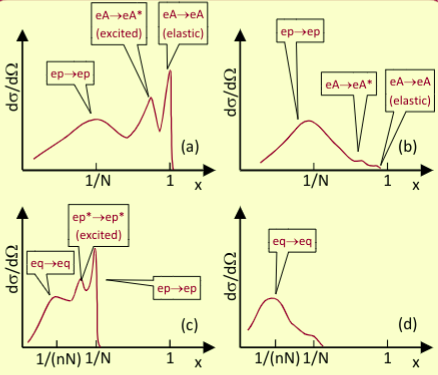
\includegraphics[width=0.6\textwidth]{immagini/fig_sez_urto_x.png}
        \caption{Sezione d'urto in funzione di $x=\frac{Q^2}{2M\nu}$. Non sono dati veri.}
        %\label{}
    \end{figure}
    \item Da (a) a (d), $Q^2$ aumenta:
    \begin{enumerate}[label=(\alph*)]
        \item A piccoli $Q^2$ ci sono scattering sia con i nuclei sia con i nucleoni.
        \item Aumentando $Q^2$, lo scattering $eN$ scompare mentre lo scattering $ep$ rimane costante.
        \item Aumentando $Q^2$, i costituenti, se presenti, appaiono come $eq\to eq$.
        \item Infine per $Q^2$ molto grandi, il processo più importante (l'unico) è $eq\to eq$.
    \end{enumerate}
\end{itemize}
\subsubsection{Vediamo i costituenti}
Con DESY (1968) si studiò lo scattering $ep\to eX$.
\begin{figure}[H]
    \centering
    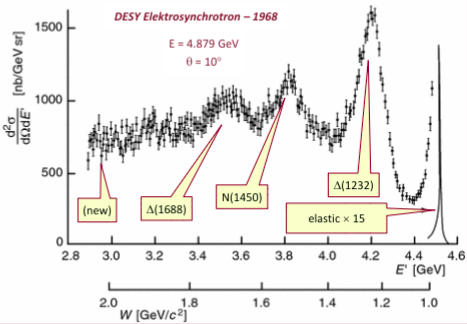
\includegraphics[width=0.6\textwidth]{immagini/fig_desy_1968.png}
    %\caption{Distribuzione complessa dello scattering $ep\to eX$ a DESY nel 1968.}
    %\label{}
\end{figure}
\begin{itemize}
    \item Si usarono elettroni di energia pari a circa 5 GeV, maggiore di quella dello SLAC.
    \item Delle risonanze del tipo $ep\to eR$ furono osservate.
    \item Si osservò una nuova regione a bassa $E'$ (alta $W$). In questa regione c'era:
    \begin{itemize}
        \item Del continuo senza picchi;
        \item Una ricca produzione di adroni;
        \item Nessuna nuova particella, solo protoni neutroni e pioni. Il protone si rompe in modo diverso dal nucleo ma non appare alcun costituente;
        \item I costituenti, se presenti, non appaiono come particelle libere.
    \end{itemize}
    \item Ma allora i quark esistono? Sono confinati? Perché? Qui venne proposto il colore senza averlo compreso del tutto, la QCD ancora non esisteva.
\end{itemize}
\subsection{Deep inelastic scattering}
Abbiamo la solita parametrizzazione della sezione d'urto nella regione di DIS con la formula:
\begin{gather*}
\qty(\pdv{\sigma}{\Omega}{E'})\_{DIS}=\qty(\dv{\sigma}{\Omega})\_{Mott}\qty[W_2(Q^2,\nu)+2W_1(Q^2,\nu)\tan^2\frac\vartheta2]=\\
=\frac{4Z^2\alpha^2(\hbar c)^2E'^2}{\abs{qc}^4}\cos\frac\vartheta2\qty[W_2(Q^2,\nu)+2W_1(Q^2,\nu)\tan^2\frac\vartheta2]=\\
=\frac{4\alpha^2E'^2}{Q^4}\times\qty[W_2(Q^2,\nu)\cos^2\frac\vartheta2+2W_1(Q^2,\nu)\sin^2\frac\vartheta2]
\end{gather*}
\begin{itemize}
    \item La sezione d'urto inelastica richiede due variabili per lo stato finale; poiché $Q^2$ e $\nu$ sono lorentz-invarianti, sono convenienti da usare.
    \item $W_1$ e $W_2$ sono combinazioni di $G_E$ e $G_M$ per DIS; qualche volta si usa una normalizzazione diversa:
    \begin{gather*}
    F_1(x,Q^2)=MW_1(Q^2,\nu)\\
    F_2(x,Q^2)=\nu W_2(Q^2,\nu)
    \end{gather*}
    \item La dinamica dello scattering dipende dalla struttura del bersaglio. $W_{1,2}(F_{1,2})$ sono i contenitori della informazione. 
    \item Sono note come \textit{funzioni di struttura} e devono essere misurate (o calcolate con teorie particolarmente profonde).
    \item Non c'è particolare differenza tra $W_{1,2}$ e $F_{1,2}$, quindi si usano le più convenienti. Oggi nei paper ad alti $\sqrt s$ si usano solo $F_{1,2}$.
\end{itemize}
\subsubsection{Riassunto formule}
Riassunto delle formule della sezione d'urto dei nucleoni: sezioni d'urto di Mott e Rosenbluth, e relazioni tra $G_{E,M}$ e $W_{1,2}/F_{1,2}$.
\begin{align*}
    &\qty(\dv{\sigma}{\Omega})\_{Mott} = \qty(\frac{4 \alpha^2 E'^2}{Q^4})\_{Ruth} \qty(\cos^2 \frac{\vartheta}{2})_{\to\text{Mott}^*} \qty(\frac{E'}E)_{\to\text{Mott}}=\frac{4\alpha^2 E'^3}{E Q^4} \cos^2 \frac{\vartheta}{2};\\
    &\qty(\dv{\sigma}{\Omega})\_{Rosenbluth}= \qty(\frac{4 \alpha^2 E'^3}{E Q^4}\cos^2\frac\vartheta2)\_{Mott} \qty( \frac{G_E^2 + \tau G_M^2}{1+\tau} + 2 \tau G_M^2 \tan^2 \frac{\vartheta}{2})_{\to\text{Rosenbluth}};\\
    &\qty(\pdv{\sigma}{\Omega}{E'})\_{Rosenbluth}= \frac{12 \alpha^2 E'^2}{E Q^4} \left( \frac{G_E^2 + \tau G_M^2}{1+\tau} \cos^2 \frac{\vartheta}{2} + 2 \tau G_M^2 \sin^2 \frac{\vartheta}{2} \right);\\
    &\qty(\pdv{\sigma}{\Omega}{E'})\_{DIS}= \frac{4 \alpha^2 E'^2}{Q^4}\times \left[ W_2(Q^2, \nu) \cos^2 \frac{\vartheta}{2} + 2 W_1(Q^2, \nu) \sin^2 \frac{\vartheta}{2} \right];\\
    &W_1(Q^2, \nu) = \frac{F_1(x, y)}{M} = \frac{3}{E} \tau G_M^2 = \frac{3 Q^2}{4 E M_p^2} G_M^2;\\
    &W_2(Q^2, \nu) = \frac{F_2(x, y)}{\nu} = \frac{3}{E} \left( \frac{G_E^2 + \tau G_M^2}{1 + \tau} \right) = \frac{3}{E} \left( \frac{4 M_p^2 G_E^2 + Q^2 G_M^2}{4 M_p^2 + Q^2} \right).
\end{align*}
Notiamo che 
\begin{align*}
&(Q,\nu,M)\sim E^1\\
&(\tau,G_{E,M},F_{1,2})\sim E^0\\
&W_{1,2}\sim E^{-1}\\
&\sigma,\dv{\sigma}{\Omega}\sim E^{-2}\\
&G_{E,M},F_{1,2},W_{1,2}=f(Q^2)
\end{align*}
Notiamo che le sezioni d'urto di Rutherford, di Mott e di Mott* non dipendono dalla massa del protone. Invece la sezione d'urto di Rosenbluth dipende da $\tau$ (=$\frac{Q^2}{4M^2}$) più qualunque dipendenza nascosta in $G_{E,M}$. Le $F_{1,2}$ neanche dipendono da essa.
RIASCOLTA DA NPP29 31:30